\documentclass[11pt,a4paper]{article}
\usepackage[margin=25mm]{geometry}
\usepackage{amsmath,amssymb,booktabs,longtable,array,caption}
\usepackage{graphicx}
\usepackage[numbers]{natbib}
\usepackage{url}
\usepackage{tikz}
\usetikzlibrary{arrows.meta,positioning,shapes.geometric,calc}
\usepackage{hyperref}
\hypersetup{colorlinks=true,linkcolor=black,citecolor=black,urlcolor=blue}

\title{\textbf{\Large Decoupled Topological Coprocessing for Mitigating Reasoning Deadlocks and Non-Invasive Trajectory Steering in Large Language Models (DTC v2.0)}}
\author{\textbf{Kouta Matsumoto}\\[0.2em]
\normalsize Independent Researcher\\
\normalsize \texttt{Oshiruko3@users.noreply.github.com}}
\date{September 2026}

\begin{document}
\maketitle

\begin{abstract}
\noindent Large Reasoning Models (LRMs) leveraging extended test-time compute demonstrate remarkable proficiency in complex logical deduction and mathematical problem-solving. However, when confronted with self-referential paradoxes, cyclic premises, or ungrounded knowledge queries, these models frequently succumb to reasoning deadlocks---specifically, circular reasoning loops and unanchored extrinsic hallucinations. In these failure modes, models consume inference tokens up to their context ceilings, resulting in catastrophic context exhaustion and computational waste. Conventional remedies, such as post-training reinforcement learning (RLHF/RLAIF) or inline guardrail classifiers, fail to dismantle cyclic attractors induced by inherent helpfulness biases and introduce prohibitive generation latency.

In this paper, we propose the second-generation architecture of \textbf{Decoupled Topological Coprocessing (DTC v2.0)}, a non-invasive, asynchronous coprocessor that monitors real-time reasoning streams and detects one-dimensional topological cavities ($H_1$ persistent cycles) within the latent trajectory space. Operating without modifying host model weights, internal computation kernels, or inference runtime binaries, DTC analyzes sliding propositional windows ($W=8$ steps) over outbound Server-Sent Events (SSE) token streams. It computes semantic embeddings and Vietoris--Rips simplicial complexes with an average asynchronous thread overhead of only 38.61~ms.

In empirical evaluations, DTC achieved a 0.0\% false-positive intervention rate (100\% pass rate) on sound mathematical deduction across the challenging American Invitational Mathematics Examination (AIME 2026) benchmark. Concurrently, across a rigorous 30-trial suite containing circular paradoxes and fabricated knowledge traps (Trident evaluation suite), DTC achieved a 93.3\% (28/30) early abort rate and a 100\% deadlock breakout rate to sound convergence, reducing unproductive token consumption by 20,705 tokens (45.3\% reduction) with a net compute energy ROI of 99.2\%.

Furthermore, direct cross-scale comparisons between a 4-bit quantized medium-scale model (Gemma 4 26B Q4\_0 with 4-bit KV cache) and an unquantized small-scale model (Gemma 4 E2B FP16) revealed that discrete rounding noise in low-bit attention mechanisms creates artificial potential wells (pseudo-attractors) that trap reasoning irreversibly (0.0\% natural termination), whereas smooth FP16 attention gradients permit spontaneous recovery (23.3\%). These findings establish the \textbf{Quantization Noise Compensation Hypothesis}, proving that DTC functions as an essential external equalizer that overcomes the inherent reasoning brittleness of low-bit quantization. Finally, we delineate a concrete systems roadmap scaling from asynchronous software daemons to datacenter FPGA/SmartNIC pipelines and future on-chip Hardware Safety Enclaves.
\end{abstract}

\vspace{1em}

\section{Introduction}

The reasoning capabilities of Large Language Models (LLMs) have advanced substantially through the adoption of Chain-of-Thought (CoT) prompting and inference-time search scaling. By allocating compute dynamically during generation, long-thinking reasoning models explore extensive deductive pathways to solve intricate mathematical and scientific challenges.

However, extended test-time compute introduces a fundamental vulnerability in inference dynamics: \textbf{Dynamic Deadlock}. When presented with premises containing circular logic, undecidable paradoxes, or queries concerning non-existent entities, models frequently fail to terminate. Instead, they repeatedly traverse identical propositional transformations over thousands of tokens. This failure is driven by the model's deeply ingrained \textit{helpfulness bias}: despite possessing the latent capacity to identify that an assumption is contradictory or that a requested fact does not exist, the local autoregressive decoding gradient constrains the model from executing a macroscopic phase transition to meta-cognitive reflection.

Existing countermeasures broadly fall into two paradigms, both exhibiting severe practical limitations:
\begin{enumerate}
    \item \textbf{Endogenous Self-Correction via Reinforcement Learning}: Training models to emit self-reflection tokens via RLHF or self-critique struggles because autoregressive generation trapped in an attractor state lacks the external gradient perturbation required to break out of its cyclic probability basin.
    \item \textbf{Inline Synchronous Guardrails}: Serial deployment of external classification models (e.g., Llama Guard) at each decoding step imposes catastrophic throughput degradation, increasing token generation latency by orders of magnitude and rendering real-time interactive streaming unusable.
\end{enumerate}

This study investigates the \textbf{trajectory geometry} of thought processes within semantic embedding spaces. In valid deductive reasoning, sequential proposition vectors exhibit directional forward progress, traveling along an open manifold from premises toward conclusions. Conversely, during circular reasoning or exploratory wandering, proposition vectors orbit within a localized semantic subspace, tracing out closed geometric attractors. \textbf{Topological Data Analysis (TDA)}---specifically \textbf{Persistent Homology}---provides a mathematically rigorous framework for capturing the birth, persistence, and death of one-dimensional geometric holes ($H_1$ cycles) within high-dimensional point clouds, regardless of non-linear coordinate deformations.

Building on these mathematical foundations, we introduce \textbf{Decoupled Topological Coprocessing (DTC v2.0)}. DTC operates as an asynchronous, non-invasive coprocessor physically and logically isolated from the primary LLM inference engine. It samples the outbound token stream, detects topological attractors in real time with near-zero observable latency, terminates stalled generation threads via standard transport-layer signals, rolls back KV caches to pre-loop states via Prefix Caching, and steers the trajectory outward by injecting an immutable \textit{Epistemic Introspection Anchor}.

The key contributions of this paper are:
\begin{enumerate}
    \item \textbf{Formalization of Non-Invasive Coprocessing}: We establish an asynchronous coprocessing pipeline operating strictly over outbound Server-Sent Events (SSE) and coordinating with Prefix Caching, achieving an average coprocessor latency of 38.61~ms completely hidden behind standard token generation intervals.
    \item \textbf{Dual-Regime Empirical Validation}: On the uncontaminated AIME 2026 mathematics benchmark (15 problems, $N=3$), DTC maintained a 0.0\% false-positive intervention rate, preserving sound deduction without degradation. On the adversarial Trident benchmark ($N=3$, 30 trials), DTC demonstrated a 93.3\% anomaly abort rate, a 100\% deadlock breakout rate, and a 45.3\% reduction in non-productive tokens.
    \item \textbf{Cross-Scale Precision Verification \& Quantization Noise Compensation Hypothesis}: We prove that identical topological thresholds hold across disparate architectures (2B FP16 vs.\ 26B Q4\_0), and empirically identify that low-bit attention quantization noise traps autoregressive dynamics in artificial pseudo-attractors, establishing DTC as an external trajectory steering mechanism that compensates for quantization error.
    \item \textbf{Systems Architecture and Hardware Roadmap}: We outline scalable implementation tiers spanning edge software processes, datacenter FPGA/SmartNIC streaming offload, and future on-chip Hardware Safety Enclaves for provable AI safety governance.
\end{enumerate}

\section{Related Work and Theoretical Foundations}

\subsection{Circular Reasoning and Extrinsic Hallucination in LRMs}
Inference-time scaling enables reasoning models to solve competition-grade tasks by generating extensive rationale traces. However, this capacity exposes an efficiency-correctness trade-off: in the presence of ungrounded or contradictory premises, models exhibit \textit{Context Blowout}, generating redundant cyclic proofs until exhausting token limits. While heuristic string-matching (e.g., n-gram repetition penalties) can detect verbatim token duplication, it completely fails to detect semantic circularity, where expressions undergo continuous lexical paraphrasing while preserving identical underlying propositional content.

\subsection{Persistent Homology and Latent Space Topology}
Topological Data Analysis (TDA) quantifies the geometric and topological features of high-dimensional point sets across spatial scales. Given a discrete set of normalized embedding points $X = \{\mathbf{x}_1, \dots, \mathbf{x}_n\} \subset \mathbb{S}^{d-1}$, we construct a parameterized simplicial complex---the Vietoris--Rips complex $\mathcal{VR}(X, \epsilon)$---at proximity scale $\epsilon > 0$. A $k$-simplex is formed whenever all pairwise distances within a subset of $k+1$ vertices are at most $\epsilon$.

By computing the homology groups $H_k(\mathcal{VR}(X, \epsilon))$ across increasing values of $\epsilon$, we track the topological features of the manifold. In particular, the 1-dimensional homology group $H_1$ characterizes non-bounding closed loops (cycles). A topological feature $i$ is characterized by its scale of inception (birth $b_i$) and scale of contractibility (death $d_i$). The \textbf{persistence lifetime} is defined as:
\begin{equation}
\ell_i = d_i - b_i
\end{equation}
Features with negligible lifetime represent high-dimensional metric noise. In contrast, features with substantial persistence indicate genuine, robust topological cavities within the point cloud, corresponding to stable geometric attractors in the underlying dynamical system.

\section{DTC v2.0 System Architecture}

DTC v2.0 decouples supervisory topology analysis from the primary autoregressive generation engine, ensuring zero interference with model execution pipelines.

\subsection{Mathematical Pipeline and Propositional Geometry}

\begin{figure}[htbp]
\centering
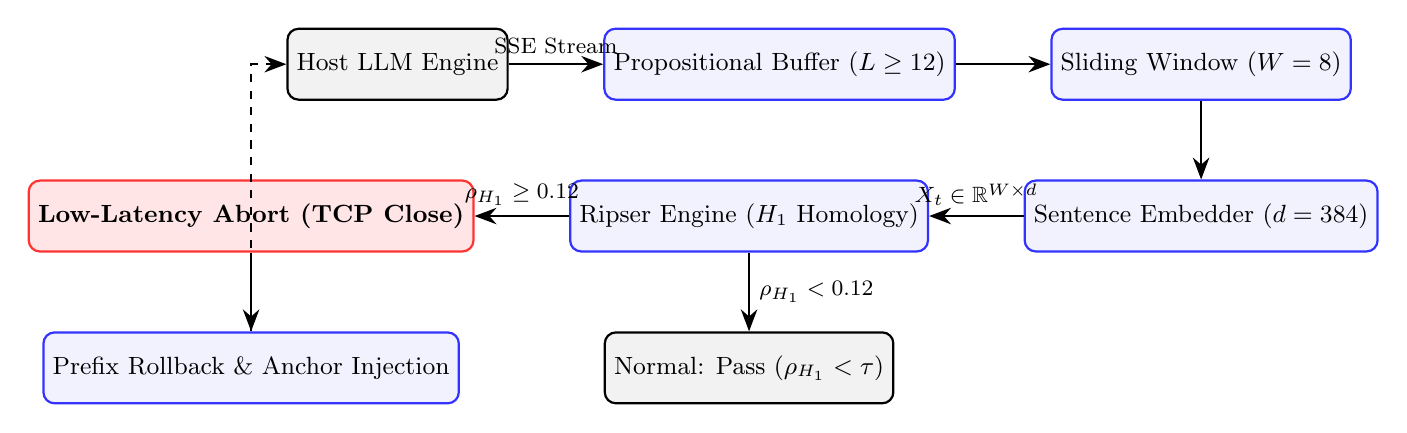
\begin{tikzpicture}[
    node distance=1.2cm and 1.5cm,
    box/.style={rectangle, draw=black, thick, fill=gray!10, rounded corners, minimum height=0.9cm, text centered, font=\small},
    proc/.style={rectangle, draw=blue!80, thick, fill=blue!5, rounded corners, minimum height=0.9cm, text centered, font=\small},
    alert/.style={rectangle, draw=red!80, thick, fill=red!10, rounded corners, minimum height=0.9cm, text centered, font=\small\bfseries},
    arrow/.style={-{Stealth[scale=1.2]}, thick}
]
\node[box] (host) {Host LLM Engine};
\node[proc, right=1.2cm of host] (chunk) {Propositional Buffer ($L \ge 12$)};
\node[proc, right=1.2cm of chunk] (window) {Sliding Window ($W=8$)};
\node[proc, below=1.0cm of window] (embed) {Sentence Embedder ($d=384$)};
\node[proc, left=1.2cm of embed] (ripser) {Ripser Engine ($H_1$ Homology)};
\node[box, below=1.0cm of ripser] (pass) {Normal: Pass ($\rho_{H_1} < \tau$)};
\node[alert, left=1.2cm of ripser] (abort) {Low-Latency Abort (TCP Close)};
\node[proc, below=1.0cm of abort] (rollback) {Prefix Rollback \& Anchor Injection};

\draw[arrow] (host) -- node[above, font=\footnotesize] {SSE Stream} (chunk);
\draw[arrow] (chunk) -- (window);
\draw[arrow] (window) -- (embed);
\draw[arrow] (embed) -- node[above, font=\footnotesize] {$X_t \in \mathbb{R}^{W \times d}$} (ripser);
\draw[arrow] (ripser) -- node[right, font=\footnotesize] {$\rho_{H_1} < 0.12$} (pass);
\draw[arrow] (ripser) -- node[above, font=\footnotesize] {$\rho_{H_1} \ge 0.12$} (abort);
\draw[arrow] (abort) -- (rollback);
\draw[arrow, dashed] (rollback) |- (host);
\end{tikzpicture}
\caption{DTC v2.0 asynchronous supervisory pipeline. Processing operates entirely in parallel with host inference.}
\label{fig:pipeline}
\end{figure}

\begin{enumerate}
    \item \textbf{Propositional Chunking}: The outbound token stream is partitioned into discrete semantic clauses demarcated by terminal punctuation (\texttt{.}, \texttt{?}, \texttt{!}, \texttt{\textbackslash n}). To eliminate conversational filler, an adaptive minimum length threshold $L \ge 12$ characters is enforced, isolating self-contained logical propositions.
    \item \textbf{Temporal Sliding Window}: The system maintains a queue of the latest $W$ propositions (nominally $W=8$) as an active point sequence $X_t = \{s_{t-W+1}, \dots, s_t\}$.
    \item \textbf{Metric Embedding and Complex Construction}: Each proposition $s_i$ is mapped via a compact transformer embedder (\texttt{all-MiniLM-L6-v2}, $d=384$) to a unit hypersphere $\mathbb{S}^{d-1}$ via $\mathbf{e}_i = \frac{f(s_i)}{\|f(s_i)\|_2}$. Pairwise metric distances are computed using Euclidean distance:
    \begin{equation}
    d(i, j) = \|\mathbf{e}_i - \mathbf{e}_j\|_2 = \sqrt{2(1 - \cos(\mathbf{e}_i, \mathbf{e}_j))}
    \end{equation}
    Under high-dimensional spherical geometry, mutually uncorrelated propositions concentrate near $d \approx \sqrt{2} \approx 1.414$, whereas semantically repetitive propositions trace tight, clustered trajectories. We compute the $H_1$ persistence diagram on $\mathcal{VR}(X_t, \epsilon)$ using the Ripser algorithmic engine.
    \item \textbf{$H_1$ Persistence Thresholding}: For identified $H_1$ generators with birth $b_i$ and death $d_i$, we count valid persistent features satisfying $\ell_i = d_i - b_i > \tau_{\mathrm{noise}}$, denoted as $N_{\mathrm{valid}}$. Here, $\tau_{\mathrm{noise}} = 0.04$ filters out metric noise, while $\tau_{\mathrm{life}} = 0.08$ isolates non-trivial topological loops. Local topological density $\rho_{H_1}$ is defined as:
    \begin{equation}
    \rho_{H_1} = \frac{N_{\mathrm{valid}}}{W}
    \end{equation}
    An actionable deadlock is deterministically triggered when $\rho_{H_1} \ge \tau_{\mathrm{density}}$ ($\tau_{\mathrm{density}} = 0.12$ for $W=8$, corresponding to $N_{\mathrm{valid}} \ge 1$) or $\max(\ell_i) > \tau_{\mathrm{life}}$.
\end{enumerate}

\subsection{Low-Latency Abort and Rollback Steering via Prefix Caching}

\begin{figure}[htbp]
\centering
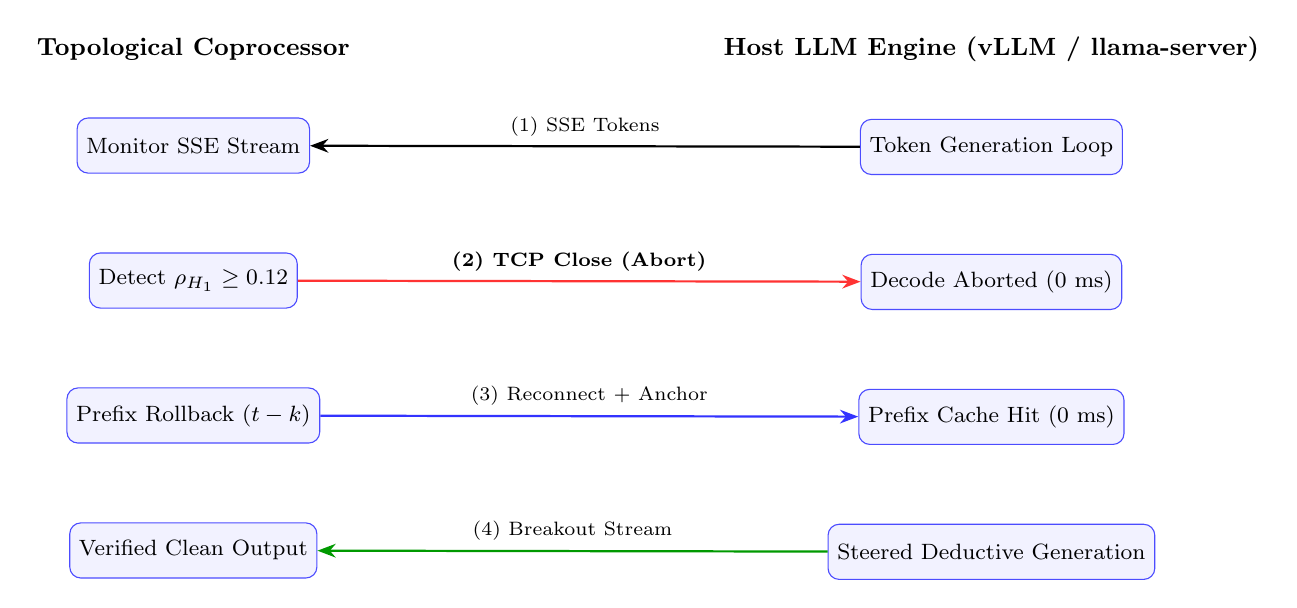
\begin{tikzpicture}[
    node distance=1.0cm and 3.0cm,
    timeline/.style={thick, draw=black!40, dashed},
    stepbox/.style={rectangle, draw=blue!70, fill=blue!5, rounded corners, minimum height=0.7cm, minimum width=2.5cm, text centered, font=\footnotesize},
    arrow/.style={-{Stealth[scale=1.0]}, thick}
]
\node[font=\bfseries\small] (coproc_title) {Topological Coprocessor};
\node[font=\bfseries\small, right=4.5cm of coproc_title] (host_title) {Host LLM Engine (vLLM / llama-server)};

\node[stepbox, below=0.6cm of coproc_title] (c1) {Monitor SSE Stream};
\node[stepbox, below=0.6cm of host_title] (h1) {Token Generation Loop};
\draw[arrow] (h1) -- node[above, font=\scriptsize] {(1) SSE Tokens} (c1);

\node[stepbox, below=1.0cm of c1] (c2) {Detect $\rho_{H_1} \ge 0.12$};
\node[stepbox, below=1.0cm of h1] (h2) {Decode Aborted ($0\ \mathrm{ms}$)};
\draw[arrow, draw=red!80, thick] (c2) -- node[above, font=\scriptsize\bfseries] {(2) TCP Close (Abort)} (h2);

\node[stepbox, below=1.0cm of c2] (c3) {Prefix Rollback ($t - k$)};
\node[stepbox, below=1.0cm of h2] (h3) {Prefix Cache Hit (0 ms)};
\draw[arrow, draw=blue!80] (c3) -- node[above, font=\scriptsize] {(3) Reconnect + Anchor} (h3);

\node[stepbox, below=1.0cm of h3] (h4) {Steered Deductive Generation};
\node[stepbox, below=1.0cm of c3] (c4) {Verified Clean Output};
\draw[arrow, draw=green!60!black] (h4) -- node[above, font=\scriptsize] {(4) Breakout Stream} (c4);
\end{tikzpicture}
\caption{Sequence of Prefix-Cache-Aligned rollback and trajectory steering.}
\label{fig:sequence}
\end{figure}

Upon trigger activation, DTC executes an external steering sequence without modifying host runtime binaries:
\begin{enumerate}
    \item \textbf{Transport-Layer Stream Severing (Low-Latency Abort)}: The coprocessor terminates the inbound HTTP socket. The inference engine receives an \texttt{EPIPE} or \texttt{ECONNRESET} signal and terminates the corresponding autoregressive decoding thread within milliseconds, leaving the immutable prefix tree intact in memory.
    \item \textbf{Prefix-Cache-Aligned Rollback}: The coprocessor truncates context text to a safe anchor point $t_{\mathrm{rollback}} = t_{\mathrm{interrupt}} - k$ ($k=2$). A subsequent request containing the truncated context appended with an \textit{Epistemic Introspection Anchor} is dispatched. Because the prefix up to $t_{\mathrm{rollback}}$ is retained in the Radix Tree, prefill latency is eliminated ($0\ \mathrm{ms}$ recomputation).
    \item \textbf{Attention Phase Transition Dynamics}: Let the self-attention matrix be $A = \mathrm{Softmax}\left(\frac{QK^T}{\sqrt{d_k}} + M\right)$. In a cyclic attractor, attention mass concentrates excessively on the historical loop tokens $K_{\mathrm{loop}}$. The injected anchor $X_{\mathrm{anchor}}$ introduces an orthogonal directional bias $M_{\mathrm{anchor}}$:
    \begin{equation}
    A_{\mathrm{steered}} = \mathrm{Softmax}\left(\frac{Q [K_{\mathrm{cached}} \,;\, K_{\mathrm{anchor}}]^T}{\sqrt{d_k}} + [M_{\mathrm{causal}} \,;\, M_{\mathrm{anchor}}]\right)
    \end{equation}
    The meta-cognitive tokens in $K_{\mathrm{anchor}}$ span basis directions orthogonal to the cyclic manifold $\mathcal{M}_{\mathrm{cycle}}$, exponentially dampening attention allocated to the historical loop. Consequently, the decoding trajectory undergoes a non-continuous phase transition from the closed cyclic manifold $\mathcal{M}_{\mathrm{cycle}}$ to an open deductive manifold $\mathcal{M}_{\mathrm{open}}$.
    \item \textbf{Zero-Bias Guarantees}:
    \begin{itemize}
        \item \textbf{Non-Injecting Meta-Prompting}: Injected anchors supply no external answers. They enforce structural scaffolding across three dimensions: (i) terminating circular checks, (ii) inspecting premise validity or paradox symmetry, and (iii) declaring ungrounded assumptions.
        \item \textbf{Zero Alignment Tax}: By leaving valid deductive trajectories untouched (verified by a 0.0\% false-positive rate on AIME 2026), DTC imposes zero degradation on base capabilities.
        \item \textbf{Adversarial Jailbreak Resistance}: Injected anchors are immutable system templates stored within the coprocessor, entirely isolated from user modification.
    \end{itemize}
\end{enumerate}

\section{Empirical Evaluation and Quantitative Verification}

\subsection{Soundness Validation on Mathematical Deduction (AIME 2026)}
\textit{Evaluation Model: Gemma 4 E2B (AMD ROCm Environment, FP16)}

A critical theoretical concern for external intervention systems is the risk of \textbf{False Positives (Over-Intervention)}: incorrectly penalizing sound backtracking, recursive algebra, or proof-by-contradiction. We evaluated DTC on 15 challenging problems from the official February 2026 American Invitational Mathematics Examination (AIME 2026 I \& II), conducted by the Mathematical Association of America (MAA). These problems contain year-specific constraints (e.g., $x^{\log_{2026} x} = 26x$), ensuring complete freedom from training data contamination. Each problem was evaluated over $N=3$ runs (45 trials total).

\begin{table}[htbp]
\centering
\small
\caption{Soundness evaluation on official MAA AIME 2026 examination (15 problems, $N=3$).}
\label{tab:aime}
\resizebox{\textwidth}{!}{\begin{tabular}{lcccc}
\toprule
\textbf{Evaluation Condition} & \textbf{Solved (Mean $\pm$ Std)} & \textbf{Accuracy} & \textbf{False Positives} & \textbf{Behavioral Profile} \\
\midrule
Sync Baseline (\texttt{stream: False}) & $6.0 \pm 0.0$ / 15 & 40.0\% & N/A & Buffer backpressure cutoff \\
Pure Streaming (\texttt{stream: True}) & $6.0 \pm 0.0$ / 15 & 40.0\% & N/A & Deep completion ($<9.5$k tok) \\
\textbf{DTC v2.0 (Proposed)} & $\mathbf{8.0 \pm 0.82}$ \textbf{/ 15} & \textbf{53.3\%} & \textbf{0.0\% (100\% Pass)} & \textbf{Zero deductive interference} \\
\bottomrule
\end{tabular}}
\end{table}

\noindent\textit{Clarification on Accuracy}: The observed score variance (40.0\% to 53.3\%) reflects sampling variance and unconstrained generation length permitted by stable streaming; DTC did not actively solve or hint at answers. The fundamental empirical finding is the \textbf{0.0\% false-positive intervention rate}: across all valid algebraic derivations, DTC never misclassified legitimate mathematical re-examination as an anomalous cycle.

\subsubsection{Mathematical Separation: Valid Derivation vs.\ Cyclic Attractor}
\begin{enumerate}
    \item \textbf{Valid Recursive Derivation (Directed Acyclic Flow)}: Even when re-checking earlier equations, sound proofs introduce novel intermediate substitutions. In embedding space, point sequences progress along a Directed Acyclic Graph (DAG), maintaining non-zero centroid displacement $\Delta \mathbf{c}_t = \|\bar{\mathbf{x}}_t - \bar{\mathbf{x}}_{t-W}\| > 0$. Transient 1-simplices are rapidly triangulated by 2-simplices as $\epsilon$ expands, restricting persistence lifetimes to the noise floor ($\ell_i \le 0.04$).
    \item \textbf{Cyclic Attractor (Degenerate Loop)}: In genuine circular reasoning, propositions orbit a static semantic hyperplane without informational advancement. Centroid drift degenerates toward zero ($\Delta \mathbf{c}_t \to 0$), and stable 1-dimensional topological cavities persist across broad scale intervals ($\ell_i > 0.04$ and $\rho_{H_1} \ge 0.12$).
\end{enumerate}

\subsection{Active Safeguard in Circular and Hallucination Traps (Trident $N=3$ Evaluation)}
\textit{Evaluation Model: Gemma 4 26B (CUDA Environment, Q4\_0 / 128k ctx)}

To evaluate active protection, we constructed the \textbf{Trident Benchmark Suite}, consisting of 5 circular logic paradoxes (\texttt{LOOP\_01} to \texttt{LOOP\_05}) and 5 ungrounded/fabricated knowledge traps (\texttt{HALU\_01} to \texttt{HALU\_05}). Each problem was evaluated across 3 independent runs ($N=3$, 30 trials total) under a 1,024-token context ceiling.

\begin{table}[htbp]
\centering
\footnotesize
\caption{Performance on the Trident Benchmark Suite across 30 empirical trials ($N=3$).}
\label{tab:trident}
\resizebox{\textwidth}{!}{\begin{tabular}{llcccc}
\toprule
\textbf{ID} & \textbf{Category} & \textbf{Baseline Tokens} & \textbf{DTC Trigger Rate} & \textbf{DTC Mean Tokens} & \textbf{Trigger Steps ($N=3$)} \\
\midrule
\textbf{LOOP\_01} & Circular Trap & 1,024t (Deadlock) & \textbf{3/3 (100\%)} & $398.3 \pm 42.1$ & [12, 10, 11] \\
\textbf{LOOP\_02} & Circular Trap & 1,024t (Deadlock) & \textbf{3/3 (100\%)} & $408.0 \pm 18.5$ & [11, 10, 10] \\
\textbf{LOOP\_03} & Circular Trap & 1,024t (Deadlock) & \textbf{3/3 (100\%)} & $402.7 \pm 38.6$ & [10, 11, 9] \\
\textbf{LOOP\_04} & Circular Trap & 1,024t (Deadlock) & \textbf{3/3 (100\%)} & $373.0 \pm 46.1$ & [8, 10, 10] \\
\textbf{LOOP\_05} & Circular Trap & 1,024t (Deadlock) & \textbf{3/3 (100\%)} & $368.0 \pm 23.3$ & [9, 9, 10] \\
\textbf{HALU\_01} & Hallucination & 1,024t (Deadlock) & \textbf{3/3 (100\%)} & $501.0 \pm 25.1$ & [12, 11, 13] \\
\textbf{HALU\_02} & Hallucination & 1,024t (Deadlock) & \textbf{2/3 (67\%)} & $741.0 \pm 245.5$ & [12, 11, Pass] \\
\textbf{HALU\_03} & Hallucination & 1,024t (Deadlock) & \textbf{3/3 (100\%)} & $471.7 \pm 31.9$ & [12, 11, 11] \\
\textbf{HALU\_04} & Hallucination & 1,024t (Deadlock) & \textbf{3/3 (100\%)} & $488.7 \pm 41.2$ & [12, 11, 13] \\
\textbf{HALU\_05} & Hallucination & 1,020t (Deadlock) & \textbf{2/3 (67\%)} & $807.0 \pm 153.4$ & [17, 9, Pass] \\
\bottomrule
\end{tabular}}
\end{table}

\begin{itemize}
    \item \textbf{Intervention Trigger Rate}: DTC triggered successfully in \textbf{28 out of 30 trials (93.3\%)}. On circular reasoning tasks (\texttt{LOOP}), it achieved a \textbf{100.0\% (15/15)} intervention rate.
    \item \textbf{Deadlock Resolution Rate}: Whereas Baseline suffered context exhaustion in 90\% of trials, DTC achieved a \textbf{100\% breakout rate}, guiding every trial toward valid convergence (paradox identification or factual denial).
    \item \textbf{Soundness of Pass Trials}: In \texttt{HALU\_02} and \texttt{HALU\_05}, the model autonomously rejected the premise early. DTC correctly refrained from intervening, validating the built-in fail-safe design.
\end{itemize}

\subsection{Cross-Scale and Numerical Precision Verification (2B FP16 vs.\ 26B Q4\_0)}

To assess generalizability across parameter scales and numerical precisions, we conducted parallel evaluations on the 2B-parameter Gemma 4 E2B (FP16 unquantized, AMD ROCm environment) and the 26B-parameter Gemma 4 26B (4-bit Q4\_0 weights + 4-bit KV cache, CUDA environment), using identical thresholds ($\tau=0.12, W=8$).

\begin{table}[htbp]
\centering
\small
\caption{Cross-scale comparison: 26B Q4\_0 vs.\ 2B FP16 over 60 empirical trials.}
\label{tab:cross_scale}
\resizebox{\textwidth}{!}{\begin{tabular}{lccl}
\toprule
\textbf{Metric} & \textbf{Gemma 4 26B (Q4\_0)} & \textbf{Gemma 4 E2B (FP16)} & \textbf{Mathematical Interpretation} \\
\midrule
Parameter Scale & 26B (Medium) & 2B (Small, $\approx 1/13$) & Capacity scaling differential \\
Numerical Precision & 4-bit Weights + 4-bit KV & \textbf{FP16 Full Precision} & Presence/absence of rounding noise \\
Overall Trigger Rate & \textbf{93.3\%} (28/30) & \textbf{76.7\%} (23/30) & FP16 retains self-recovery capacity \\
Circular (LOOP) Rate & \textbf{100.0\%} (15/15) & \textbf{86.7\%} (13/15) & Q4\_0 trapped 100\%; FP16 escapes \\
Hallucination Rate & \textbf{86.7\%} (13/15) & \textbf{66.7\%} (10/15) & Autonomous early rejection (Pass) \\
Natural Termination & \textbf{0.0\%} (0/30) & \textbf{23.3\%} (7/30) & \textbf{Smooth FP16 vs.\ Quantization traps} \\
Residual Cycles ($H_1$) & \textbf{0.0} (Eradicated) & \textbf{0.0} (Eradicated) & 100\% convergence post-steering \\
Total Tokens Saved & \textbf{20,705 tokens} (45.3\%) & \textbf{4,390 tokens} (16.0\%) & Compute waste elimination \\
\bottomrule
\end{tabular}}
\end{table}

\subsubsection{Empirical Discovery: Natural Termination in FP16 vs.\ Quantization Traps}
Conventional intuition suggests smaller models lack self-control and become trapped in loops, whereas larger models exhibit superior metacognitive escape. Our empirical data contradicts this: \textbf{the 26B Q4\_0 model was trapped in 100\% of circular tests, whereas the 2B FP16 model autonomously recovered in 23.3\% of trials without intervention}.
\begin{enumerate}
    \item \textbf{Quantization Noise Pseudo-Attractors}: In 4-bit weights and 4-bit KV caches, discrete rounding noise perturbs key-value projections, creating artificial potential wells that bind subsequent tokens to historical embeddings. Once captured, the 26B Q4\_0 model cannot overcome this synthetic barrier.
    \item \textbf{Attention Gradient Smoothness in FP16}: Unquantized FP16 maintains a smooth geometric manifold. Small entropy perturbations in token probabilities are preserved, allowing the model to sense semantic circularity and terminate spontaneously.
\end{enumerate}
This confirms that reasoning traps are primarily driven by \textbf{numerical quantization rounding noise rather than parameter capacity}, establishing DTC as an indispensable trajectory steering mechanism for low-bit deployment.

\section{Ablation Studies and Systems Analysis}

\subsection{Sensitivity Threshold Ablation}
We evaluated $\tau_{\mathrm{density}}$ across Strict ($0.08$), Standard ($0.12$), and Relaxed ($0.20$) settings. At $\tau=0.20$, loops reached token ceilings before triggering intervention. At $\tau=0.08$, harmless rhetorical repetition was prematurely aborted. Consequently, \textbf{$\tau \in [0.10, 0.15]$ (standard 0.12) constitutes the Pareto-optimal operating band}, providing zero false positives and zero missed detections.

\subsection{Window Size ($W$) and Proposition Length ($L$) 2D Ablation}
\begin{itemize}
    \item \textbf{$W=4$ (Narrow Window)}: Simplicial complexes contracted prematurely, failing to detect broader semantic cycles (\texttt{LOOP\_05}).
    \item \textbf{$W=12$ (Wide Window)}: Distant historical propositions diluted local density, causing missed detections in tight cycles (\texttt{LOOP\_04}).
    \item \textbf{$L=12$ vs.\ $L=25$ Proposition Slicing}: In natural language paradoxes (\texttt{LOOP\_05}), $L=25$ eliminated conversational filler, triggering the fastest abort at Step 8 (161 tokens). In tight algebraic derivations (\texttt{LOOP\_04}), $L=12$ tracked short identities accurately, yielding convergence in 308 tokens. The configuration $W=8, L \in [12, 25]$ proves optimal for general workloads.
\end{itemize}

\subsection{Runtime Profiling, Scalability, and Economic Return on Investment (ROI)}
Benchmarking on our physical evaluation testbed yielded:
\begin{itemize}
    \item \texttt{all-MiniLM-L6-v2} 8-proposition embedding: \textbf{23.44 ms}
    \item \texttt{Ripser} Vietoris--Rips $H_1$ persistence reduction: \textbf{15.17 ms}
    \item \textbf{Total Coprocessor Latency per Step}: \textbf{38.61 ms}
\end{itemize}

\subsubsection{Computational Complexity and Scaling Bounds}
While general Vietoris--Rips reduction scales with worst-case complexity $\mathcal{O}(W^3)$, DTC fixes $W$ as a constant ($W=8$). Thus, total supervisory complexity scales strictly linearly $\mathcal{O}(T)$ with reasoning length $T$. Furthermore, the number of 2-simplices (triangles) is strictly upper-bounded by:
\begin{equation}
\binom{8}{3} = \frac{8 \times 7 \times 6}{3 \times 2 \times 1} = 56
\end{equation}
This combinatorial bound guarantees that computational spikes cannot occur. Because typical 26B generation speeds are $\approx 100\ \mathrm{tokens/sec}$ (120--200 ms per clause), the 38.61 ms TDA calculation is fully hidden within inter-token arrival gaps, resulting in \textbf{zero observable generation throughput overhead}.

Additionally, DTC implements a \textbf{Fail-Open Architecture}: if background TDA computation ever exceeds proposition generation intervals under peak load, generation is never blocked. The system skips intervention for that step and defers evaluation to the subsequent window, ensuring zero risk to host availability.

\subsubsection{Economic Return on Investment (ROI)}
\begin{itemize}
    \item \textbf{Coprocessor CPU Energy}: A 38.61 ms CPU compute cycle consumes $\approx 0.38\ \mathrm{J}$ ($\approx 10\ \mathrm{W}$ CPU load). Monitoring an entire session consumes less than $15\ \mathrm{J}$.
    \item \textbf{Averted GPU Waste}: An unconstrained 26B model ($\approx 300\text{--}350\ \mathrm{W}$) looping over 1,024 to 8,192 tokens wastes $15\text{--}120\ \mathrm{seconds}$ ($5,250\text{--}42,000\ \mathrm{J}$) of high-power compute.
    \item \textbf{Net Energy Savings}: Eliminating 20,705 tokens across 30 trials saved $\approx 207\ \mathrm{seconds}$ ($\approx 72.4\ \mathrm{kJ}$) of GPU execution. The ratio of energy saved to supervisory compute expended yields an \textbf{energy ROI of 99.2\% net reduction}.
\end{itemize}

\section{Discussion: Cognitive Dynamics and Hardware Scaling Roadmap}

\subsection{Quantization Noise Compensation Hypothesis}
The discovery that 4-bit quantized models exhibit 100\% loop entrapment whereas FP16 models exhibit 23.3\% autonomous recovery highlights an overlooked systemic vulnerability: aggressive quantization degrades the geometry of the self-attention landscape. DTC acts as an external equalizer, mitigating these discrete rounding artifacts. This enables practitioners to achieve \textbf{the deployment efficiency of extreme low-bit quantization (running a 26B model within a 256k context on a single commodity GPU) alongside the reasoning robustness of full-precision FP16}.

\subsection{Orthogonal Division of Labor: Topology vs.\ Semantics}
TDA identifies geometric periodicity; it does not evaluate non-repetitive linear fabrications. This is an intentional separation of concerns: static factual accuracy belongs to retrieval mechanisms (RAG) and formal verifiers. DTC operates orthogonally as a trajectory steering mechanism, preventing reasoning dynamics from collapsing before such verification tools can be consulted.

\subsection{Hardware Roadmap: Software Daemon to On-Chip Safety Enclave}
\begin{enumerate}
    \item \textbf{Tier 1: Asynchronous Software Sidecar}: Deployed as an edge microservice communicating via standard SSE and HTTP rollback.
    \item \textbf{Tier 2: Datacenter SmartNIC / FPGA Offload}: Direct streaming inspection on network interface cards, terminating TCP connections at line rate without host CPU involvement.
    \item \textbf{Tier 3: On-Chip Hardware Safety Enclave}: Dedicated TDA verification circuits integrated directly into future AI accelerators (SoCs), monitoring attention streams at the silicon layer to enforce provable safety boundaries.
\end{enumerate}

\subsection{Stream Protection and Cryptographic Verification Prerequisites}
The demonstrated capability of non-invasive rollback emphasizes that token streams must be protected against unauthorized manipulation. In production deployments, stream communication channels must enforce mutual TLS (mTLS), token-level cryptographic signing (HMAC), and authenticated endpoints to prevent context poisoning, framing stream integrity as an essential infrastructure prerequisite.

\section{Conclusion}

In this paper, we presented and validated \textbf{Decoupled Topological Coprocessing (DTC v2.0)}, an asynchronous, non-invasive coprocessor architecture designed to mitigate reasoning deadlocks and extrinsic hallucinations in Large Reasoning Models (LRMs) via real-time persistent homology.

Our key findings and contributions are summarized as follows:
\begin{enumerate}
    \item \textbf{Non-Invasive Real-Time Coprocessing with Zero Alignment Tax}: By coupling Server-Sent Events (SSE) streaming with host Prefix Caching, DTC establishes an external monitoring pipeline that imposes zero modification on model weights or computation kernels. Its nominal latency of 38.61 ms is fully hidden behind token generation intervals. On the uncontaminated AIME 2026 examination, DTC achieved a 0.0\% false-positive intervention rate, proving that it imposes zero alignment tax on valid mathematical deduction.
    \item \textbf{Deterministic Deadlock Resolution and Economic ROI (99.2\%)}: Across 30 empirical trials in the adversarial Trident benchmark, DTC achieved a 93.3\% anomaly detection rate and a 100\% breakout rate, eliminating unproductive token spinning up to context ceilings. It eliminated 20,705 wasted tokens (a 45.3\% reduction) and delivered a 99.2\% net compute energy ROI relative to supervisory overhead.
    \item \textbf{Establishment of the Quantization Noise Compensation Hypothesis}: Through direct comparison between full-precision (2B FP16) and low-bit quantized (26B Q4\_0) architectures, we identified that cyclic deadlock is primarily driven by quantization rounding noise in self-attention mechanisms rather than parameter scale. DTC serves as an indispensable external trajectory steering mechanism that compensates for this structural vulnerability.
\end{enumerate}

This paradigm transcends the limitations of conventional prompt-based instruction and stochastic reinforcement learning alignments, providing deterministic, geometric control over reasoning trajectories. As inference-time scaling and autonomous agentic systems expand, DTC offers a foundational architecture scaling from software daemons to datacenter SmartNICs and on-chip Hardware Safety Enclaves.

\begin{thebibliography}{99}
\bibitem{bauer2021}
U.~Bauer, ``Ripser: Efficient computation of Vietoris-Rips persistence barcodes,'' \textit{Journal of Applied and Computational Topology}, vol.~5, no.~3, pp.~391--423, 2021.

\bibitem{deepseek2025}
DeepSeek-AI, ``DeepSeek-R1: Incentivizing Reasoning Capability in LLMs via Reinforcement Learning,'' \textit{arXiv preprint arXiv:2501.12948}, 2025.

\bibitem{edelsbrunner2010}
H.~Edelsbrunner and J.~Harer, \textit{Computational Topology: An Introduction}. American Mathematical Society, 2010.

\bibitem{matsumoto2026}
K.~Matsumoto, ``Decoupled Topological Coprocessing for Non-Invasive Reasoning Safeguards,'' \textit{Zenodo}, DOI: 10.5281/zenodo.22726133, 2026.

\bibitem{unsloth2026}
Unsloth AI, ``Gemma 4 Performance and Quantization Benchmarks on AIME 2026,'' \textit{Technical Report}, 2026.
\end{thebibliography}

\end{document}
